\section{Partie 1}
\subsection{Schéma physique}
Pour extraire les données du schéma physique, nous avons utilisé le plugin SQLInspect sur Eclipse afin de récupérer toutes les requêtes SQL du programme. Un script python a ensuite été créé afin de pouvoir trier les différentes requêtes en fonction de mots-clefs. La combinaison des différentes requêtes de création des tables ainsi que des contrainte a mené à ce résultat. On peut y retrouver 6 clefs étrangères qui ne référencent pas toujours des champs uniques. La seule clef primaire composée est située sur la table \mintinline{java}{tiles}. On retrouve une multitude de champs qui sont nullable. Ces derniers peuvent être utilisés comme référence dans une clef étrangère.
Toutes les tables présentent des noms qui sont plutôt explicites. On comprend son utilité et les données qui y sont stockées. Il en va de même pour la majorité des noms d'attributs.
\begin{figure}[!ht]
    \centering
    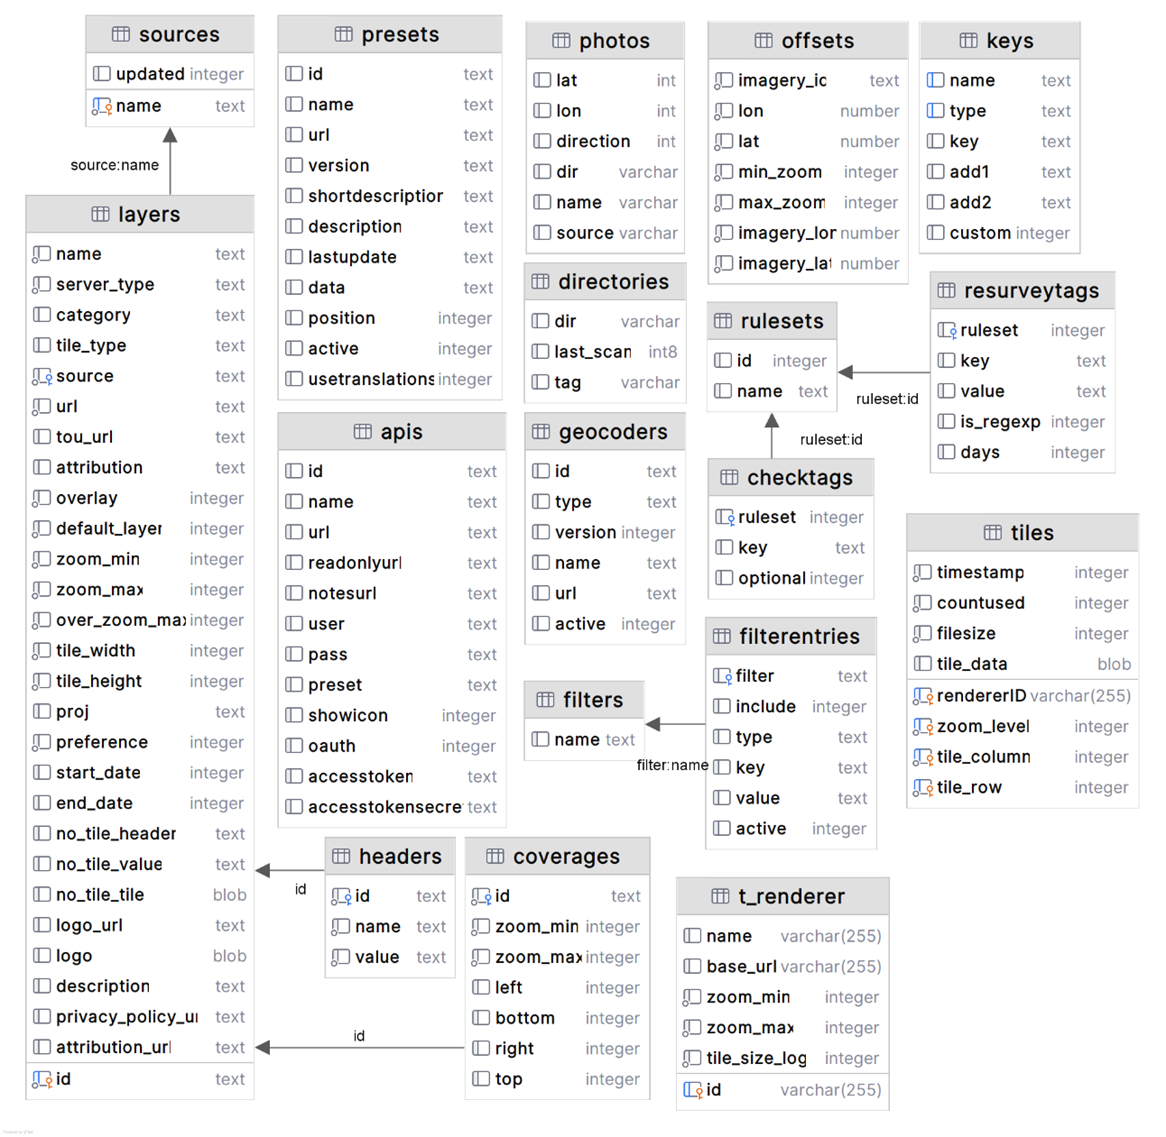
\includegraphics[scale=1]{schema_physique.png}
    \label{fig:schéma physique}
\end{figure}

\subsection{Analyse supplémentaire pour découvrir des Foreign Keys}
\subsubsection{Recherche dans le code source}
Aucune clef étrangère implicite n'a été trouvée suite à l'analyse des requêtes \mintinline{java}{SELECT} avec la regex : \mintinline{java}{(FROM|from).*,.*(WHERE|where)}. Cette dernière permet de sélectionner les requêtes qui réalisent un \mintinline{java}{SELECT} sur plusieurs tables.
Une seconde analyse des requêtes n'a donné aucun résultat pour le format de jointure SQL2. Une simple recherche du mot clef \mintinline{java}{JOIN} ne donne aucun résultat, autant dans les requêtes listées par SQLInspect ni dans le code source de l'application.

\subsubsection{Recherche de patterns}
Les tables \mintinline{java}{directories} et \mintinline{java}{photos} ont toutes les 2 un attribut « dir ». En analysant le code du fichier \mintinline{java}{PhotoIndex.java}, et plus précisément de la méthode\\\mintinline{java}{private void indexDirectories()}, on remarque qu'une query sur la table \mintinline{java}{photos} utilise la valeur de l'attribut \mintinline{java}{dir} récupéré à partir d'un select sur la table \mintinline{java}{directories}. Il y a donc un lien implicite entre ces 2 tables. Toutefois la requête utilise le mot clef \mintinline{java}{LIKE} qui permet de récupérer les entrés où l'attribut « dir » de la table \mintinline{java}{photos} contient l'attribut \mintinline{java}{dir} de la table \mintinline{java}{directories} suivi ou non d'autres caractères (symbolisé par « \% » dans la requête).

\subsection{Schéma logique}

\subsection{Schéma conceptuel}

\begin{figure}[!ht]
    \centering
    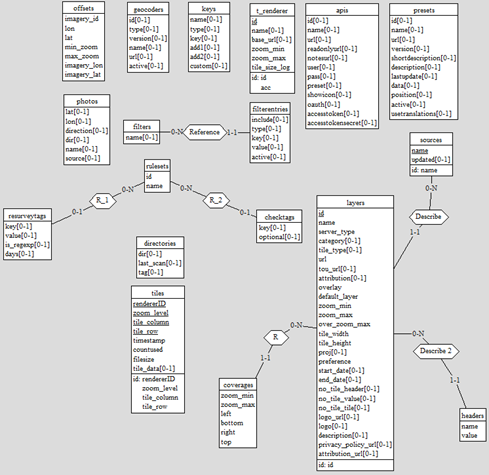
\includegraphics[scale=1]{schema_conceptuel.png}
    \label{fig:schéma conceptuel}
\end{figure}